\documentclass[12pt]{article}
\usepackage[pdftex]{graphicx}
\usepackage[inner=3cm,outer=2cm]{geometry}
\usepackage{url}
\setlength{\topmargin}{0in}
\setlength{\headheight}{0in}
\setlength{\headsep}{0in}
\setlength{\textheight}{7.7in}
\setlength{\textwidth}{6.5in}
\setlength{\oddsidemargin}{0in}
\setlength{\evensidemargin}{0in}
\setlength{\parindent}{0.15in}
\setlength{\parskip}{0.10in}

\begin{document}
%\input ../../macros/banner.tex
\rightline{V2.1~~\today}
\bigskip
\bigskip
\bigskip
\begin{center}
{\Large \bf CCERA Data Format}
\end{center}

\section{Introduction}
In this note, we propose a data format that will accomodate all or nearly all modes of data acquistion currently anticipated for the 12.8-m Carp dish.    The adoption of single format eliminates the need to specify the format for each observation and allows for the standardization of analysis code.   By archiving crucial file metadata, it makes it possible to reanalyze old datasets.  

\section{Requirements}
\begin{enumerate}
\item The format should be suitable for all presently envisaged modes of data acquistion including: transit scans, acquisition of spectral data, and pulsar observations.  
\item The data itself should be stored in binary format, readily readable by standard Python (numpy) code. 
\item File metadata, stored in plain JSON format, should be available for each data file.  
\begin{enumerate}
 \item The metadata should consist of a minimum set of required items plus an arbitrary number of additional optional items.
 \item Reading the metadata should not require advanced knowledge of the nature of the metadata.
 \end{enumerate}
 \end{enumerate}
 
 \section{Use Cases}
 As a supplement to the requirements listed above, we describe typical use cases.
 \subsection{Transit Scan}
 Here the telescope is set to a fixed azimuth and altitude, and data is taken for a prolonged period.    Since objects drift through the beam of the telescope relatively slowly, the sampling rate need not be high.   Moreover, spectral data may or may not be required.    A typical dataset might involve total run time of 1.5 hours, with a sample rate of 0.1~Hz, with each sample comprising a single total power value.  The sample size is quite small (of order 1~kByte). 
 
 \subsection{24-Hour Drift Scan}
 Again the telescope is set to a fixed azimuth and altitude and data is taken for a full day.   The objective is to see how the 21-cm signal spectrum evolves over the course of the day.  Detailed spectral information is of interest, so we assume that the spectrum has 2048 bins.  Since the evolution of the spectrum is relatively slow, one spectrum every five minutes suffices, resulting in 288 spectra for a 24-hour scan.     Two approaches to data logging are possible: i) a single file comprising 288 spectra of 2048 bins each is recorded; or ii) 288 files, each comprising a single 2048 bin spectrum, are recorded.  The total sample size is about 2.4 Mbyte for either approach. 
 
 \subsection{Pulsar Observation}
 The dish is set to track a pulsar and data is taken over an extended period (here we assume one hour) so as to average away noise.    Assuming the pulsar has a period of one second and we want to have 100 phase bins, a sample rate of at least 200~Hz is needed.    Spectral data are needed for de-dispersing the data.    Thirty-two spectral bins suffice.   Assuming a sample rate of 200~Hz and 32 spectral bins per sample, a one-hour run yields a file size of 100~Mbyte.   
 
 
 \section{Implementation}
 
 \subsection{File Names}
 Each dataset comprises two files: a binary data file and an JSON metadata file. 
 Although the metadata could be included as a header to the binary data, that 
 would involve files with mixed data types, which can be difficult to read.   Separating
 the two is ultimately simpler. 
 
 All files consist of a basename of the form {\tt YYYY-MM-DD\_HH:MM:SS\_X} and an extension, 
 which is either {\tt .raw} for data or {\tt .json} for metadata.      The time specified in the 
 basename is the UTC time at which the run begins.   The value of ``X'' is the USRP channel and 
 can be omitted if only a single channel is recorded.    
 
 \subsection{Data}
All data sets can be represented as a time series.  Each element of the series is either a single value or a power spectral density array.     The length of the time series ({\tt n\_samples}) can range from 1 to a very large number, limited only by the maximum file size (4GB?).   The spectral data take the form of a power spectral density (PSD) array (also called a ``filter bank'' array) having a variable number of bins ($N_{\rm bins}$) lying in the range $ 1 < N_{\rm bins} < 2^N$.   In principle, $N$ is unlimited but in practice will generally lie in the range $5 < N < 16$. 
Each PSD element takes the format of a 32-bit floating point number.  




% It is convenient to read and write binary data using the numpy ``{\tt .npz}'' format.   See URLs   \url{https://numpy.org/doc/stable/reference/generated/numpy.savez.html } and \url{https://numpy.org/doc/stable/reference/generated/numpy.load.html} as well as related help pages.
 
 \subsection{Metadata}
 
 The metadata file should consist of a set of entries, each consisting of a key, followed by a corresponding parameter value.   The parameter can be a string, a float, or an integer.    Strings must be enclosed by quotes, floats must contain a decimal place, and integers must consist of only digits.   Internally, the metadata take the form of a Python dictionary, which can be conveniently represented in an ASCII file using the JSON format. 

 Table~\ref{TAB1} is a list of mandatory parameters that every metadata file must contain.   The 
 order does not matter, as long as all parameters are given.   From this minimal set of parameters, 
 it is possible to reconstruct other values such as the number of FFTs that are averaged to construct 
 the PSD arrays that are saved in the file, the RA and dec in which the dish is pointing when the run starts, etc. The run\_type parameter is crucial in that it tells the system how to determine the telescope's position as time evolves: ``Transit'' means that the telescope remains at a constant azimuth and altitude, whereas ``Track'' means that the telescope moves so as to maintain a constant right acension and declination.     
 
 The selection of mandatory parameters has been done to avoid redundancy.   For example, if one knows the time and the telescope's azimuth and altitude, there is no need to specify the right 
ascension and declination, since those values can be calculated.    A set of helper functions 
can be used to compute dependent parameters---e.g., right ascension and declination---from the mandatory parameters.   
 
 \begin{table}[htbp] 
 \caption{List of mandatory metadata parameters.}
 \label{TAB1}
 \begin{center}
 \begin{tabular}{| c | c|  l |}
 \hline 
 Name & Type & Meaning \\
 \hline  \hline
t\_start        & float   & time of first sample in seconds past the epoch \\
freq      & float   & center frequency of receiver \\
srate       & float   & frequency of USRP clock in Hz \\
t\_sample     & float   & time between time series samples (or spectra) in seconds \\
n\_chans       & int  & Number of USRP channels recorded \\
fft\_size       & int     &  number channels in power spectrum \\
run\_type     & string & `Transit' or `Track' \\
az                & float  & azimuth of telescope at beginning of run in degrees \\
alt                & float  & azimuth of telescope at beginning of run in degrees \\
\hline
\end{tabular}
\end{center}
\end{table}
 
 Table~\ref{TAB2} lists optional metadata parameters.    New parameters can be added at any time.   The comment parameter is special in that multiple comments can be used.   
 
  \begin{table}[htbp] 
 \caption{List of optional metadata parameters.}
 \label{TAB2}
 \begin{center}
 \begin{tabular}{| c | c|  l |}
 \hline 
 Name & Type & Meaning \\
 \hline  \hline
run\_time & float & Run time in seconds \\
target      & string   & Astronomical object---e.g. ``Sun'' or ``M31''  \\
comment & string & text comment \\
observatory & string & Observatory name---e.g., ``Carp'' \\
run\_mode & string & Run mode---e.g., pulsar, doppler, or generic \\
RA & float & Right ascension in degrees \\
dec & float & Declination in degrees \\
gLat & float & Galactic latitude in degrees \\
gLon & float & Galactic longitude in degrees \\

\hline
\end{tabular}
\end{center}
\end{table}
 

\subsection{Reduced Data Formats}

The {\tt .raw} data format is illustrated in Fig.~\ref{FIG:format}.    Although the {\tt .raw} format contains a lot of information, the files can be inconveniently large.   In many cases, one is only interested in either a time series or a spectrum.    For example, for pulsar work at high frequencies, dispersion is often a small effect and only the time series is of interest.   In such cases, the size of the data can be reduced dramatically by summing all of the FFT bins for a given time slice into a single number.   The resulting   file, which is a simple time series,  has the extension {\tt .sum}\footnote{A possible future enhancement is a {\tt .ddsp} format, which is a de-dispersed time series.}   In other cases, only the spectral information is of interest and the size of the files can be reduced by averaging the time spectra for all time slices into a single array.    The resulting file, which is a single spectrum,  has the extension {\tt .avg}.  

\begin{figure}[htbp]
\centerline{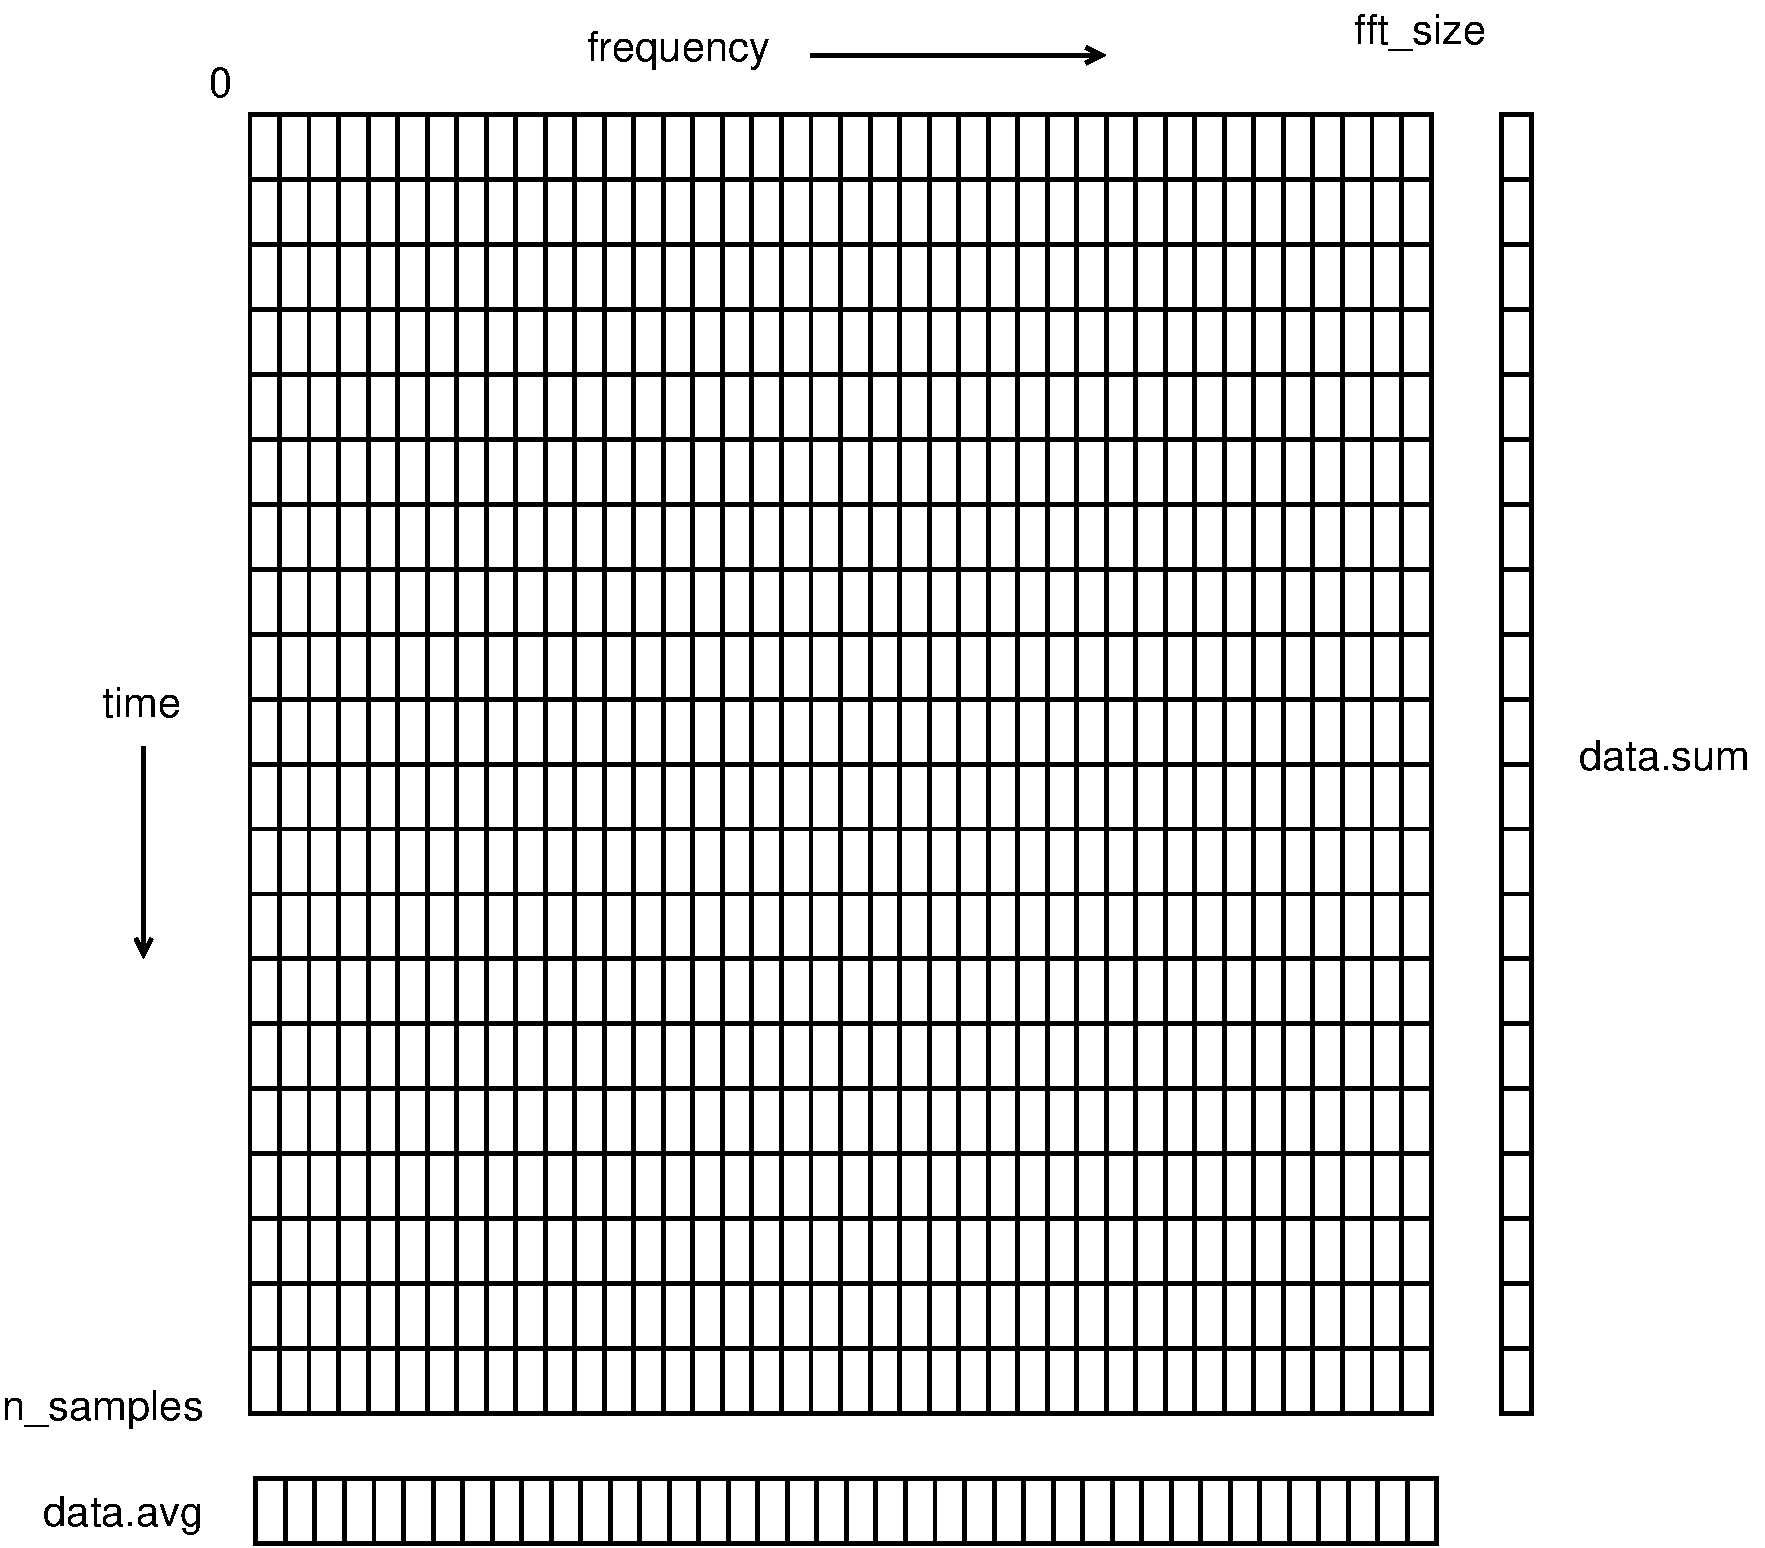
\includegraphics[width=5in]{Array.pdf}}
\caption{Graphic depiction of {\tt .raw} data format and the reduced data formats {\tt .avg} and {\tt .raw}. }
 
\label{FIG:format}
\end{figure}




\end{document}